\chapter{Data}\label{ch:Data}



\section{HMDA Data}\label{sec:HMDA_Data}

% Follow structure from presentation Ana: From where, why, which steps etc. - probably add in appendix the code for the enrichment?

The underlying data for this analysis was obtained \textit{\href{https://ffiec.cfpb.gov/data-browser/data/2022?category=states}{via the HMDA Data Browser}}. \@
All data used are structured, tabular data that are publicly available. Privacy concerns are not relevant, as the data is anonymized.

XXX UPDATE! XXX

The data was filtered to only include entries from California, as it is the largest state in the US and thus provides a high amount of data. 
The time frame was set to 2022, as it is the most recent year available (!!!!!!!!!!). No filter was applied to the financial institutions, as the analysis is not focused on the institutions themselves. 
The data was further filtered to only include entries for single-family homes, as these are the most common type of homes and therefore provide the most data.

The raw dataset resulting from these filters contains $XXX$ entries and $XXX$ features, with a total sum of loan applications amounting to $XXX$ USD. The column types are $XXX$ of numeric, and $XXX$ of object dtype. $XXX$ columns contain missing values. \@
Due to the size of the dataset, a step-by-step description of the analysis and all cleaning steps taken is too extensive for this thesis. Therefore, this chapter will only outline the key assumptions incorporated, decisions made, and steps taken for data analysis and cleaning. For full detail, please refer to the corresponding notebook at XXX.

After the initial EDA, the first step was to \textit{drop} all features that are not relevant for the analysis in order to reduce dimensionality and improve the model learning process. \@ 
In this initial step, the amount of features was reduced from $XXX$ to $XXX$ with the following reasoning:
\begin{itemize}
    \item \textbf{activity\_year}: Does not provide value as the year is already pre-filtered
    \item \textbf{lei}: Does not matter as all financial institutions are used
    \item \textbf{derived\_msa-md}: Does not matter as county code is the geographical variable used in the analysis
    \item \textbf{state\_code}: Does not matter as the state is already pre-filtered
    \item \textbf{census\_tract}: Not relevant for the analysis
    \item \textbf{derived\_dwelling\_category}: Does not matter as the building category is already pre-filtered
    \item All information regarding \textbf{co-applicants} were dropped as the focus is on the main applicant
    \item All available \textbf{Reasons for Denial} were dropped as the focus is only on \textit{if} the loan was approved
    \item The dataset contains geographical information based on census tracts. As, however, the analysis of geographical features will be based on county level, the \textbf{census tract} is dropped.
\end{itemize}

The dataset contains both actual information on protected attributes (e.g.\ \mbox{applicant\_ethnicity-1} to \mbox{applicant\_ethniciy-5}) and derived information that aggregate the former into one overarching category (e.g.\ \mbox{derived\_ethnicity}). 
As this analysis focuses on fairness concerns, where such protected attributes play an important role, the derived information is dropped in favor of the actual information in order to achieve a higher granularity of this important type of data.  
However, as only few applicants have made use of all the fields (for example, only 0.07\% of applicants have reported more than two ethnicities), the amount of features is reduced by only including the top two selections for each protected attribute. 
This is done in order to avoid a high amount of missing values in the dataset as well as to strike a balance between the amount of features (and therefore model performance) and the granularity of the data.

% Dropping of columns with high amount of NA including reasoning (add one or two pictures from missingno)
% Handling of other columns with a lot of NA
% Exempt: Reasoning for imputation, procedure, graphs
% Remove initial outliers to check distribution for initial imputation - comment on distributions
% Data Types: Except inferral and categorization


\section{Enrichment Data}\label{sec:Enrichment_Data}

% Follow structure from presentation Ana: From where, why, which steps etc. - probably add in appendix the code for the enrichment?

The enrichment data was obtained from the \textit{\href{https://www.ers.usda.gov/data-products/county-level-data-sets/}{USDA ERS page}}. All data used are structured, tabular data that are publicly available. Privacy concerns are not relevant, as the data is anonymized and aggregated. All available reports were downloaded, specifically the following datasets:

\begin{itemize}
    \item \textbf{Poverty} (2021 latest)
    \item \textbf{Population} (2022 latest)
    \item \textbf{Unemployment, and Median Household Income} (annual average 2022 unemployment and 2021 median income latest)
    \item \textbf{Education} (2017–21, 5-year average latest).
\end{itemize}

In order to clean and reshape the data in a easily analyzable format, the following steps were taken\footnote{For all detail, see the corresponding cleaning notebook at !!! XXX !!!}:
All datasets were \textit{filtered} to only contain CA county-level data, not the aggregated values for the full state of California and, in case multiple years of analysis were available, to only include the newest datapoints. 
Where there were more features available than would be useful for the analysis, the datasets were \textit{reduced} to only include the most relevant features, being:

\begin{itemize}
    \item \textbf{Poverty:} Only the percentage of the population living in poverty (PCTPOVALL\_2021) was included
    \item \textbf{Population:} Only the total population (POP\_ESTIMATE\_2022) was included
    \item \textbf{Unemployment, and Median Household Income:} The unemployment rate (Unemployment\_rate\_2022) and the median household income (Median\_Household\_Income\_2021) were included
    \item \textbf{Education:} All relative values, i.e.\ percentages of adults with their corresponding highest degrees were included.
\end{itemize}

All datasets were \textit{pivoted} in order to use the attributes as feature names and \textit{indexed} by the FIPS code and the name of the respective county. After basic \textit{checks for completeness}, the feature columns were \textit{renamed} for clarity. Finally, all datasets were \textit{merged} into a single dataframe, which was then \textit{exported} as a pickle file for further use in the analysis.

% Reasoning!

The cleaned data are \textit{complete} in a way that there are values available for all features and for all of the 58 counties. Basic summary statistics can be found in \textbf{Table \ref{tab:enrichment_summary}}. Expectedly, there is a high correlation between some of the features, see \textbf{Figure \ref{fig:CH03_Enrichment_Correlation}}.

\begin{table}[h]
    \centering
    \begin{tabularx}{\textwidth}{llllll}
    \hline
     & \textbf{Count} & \textbf{Mean} & \textbf{Std} & \textbf{Min} & \textbf{Max} \\
    \hline
    College Degree (Perc.) & 58.00 & 33.19 & 5.77 & 17.89 & 44.23 \\
    \hline
    Bachelor Degree or Higher (Perc.) & 58.00 & 28.55 & 12.27 & 11.77 & 60.15 \\
    \hline
    High School Degree (Perc.) & 58.00 & 23.77 & 5.84 & 10.17 & 38.42 \\
    \hline
    Less than High School Degree (Perc.) & 58.00 & 14.49 & 7.02 & 4.87 & 29.65 \\
    \hline
    Population (thousands) & 58.00 & 672.92 & 1,428.89 & 1.19 & 9,721.14 \\
    \hline
    Poverty Rate (Perc.) & 58.00 & 13.63 & 3.96 & 6.60 & 21.90 \\
    \hline
    Median Household Income (thousands) & 58.00 & 75.30 & 21.89 & 45.51 & 141.16 \\
    \hline
    Unemployment Rate (Perc.) & 58.00 & 4.84 & 2.07 & 2.40 & 14.70 \\
    \hline
    \end{tabularx}
    \caption{Summary Statistics of the Enrichment Data}
    \label{tab:enrichment_summary}
\end{table}

\begin{figure}[h]
    \centering
    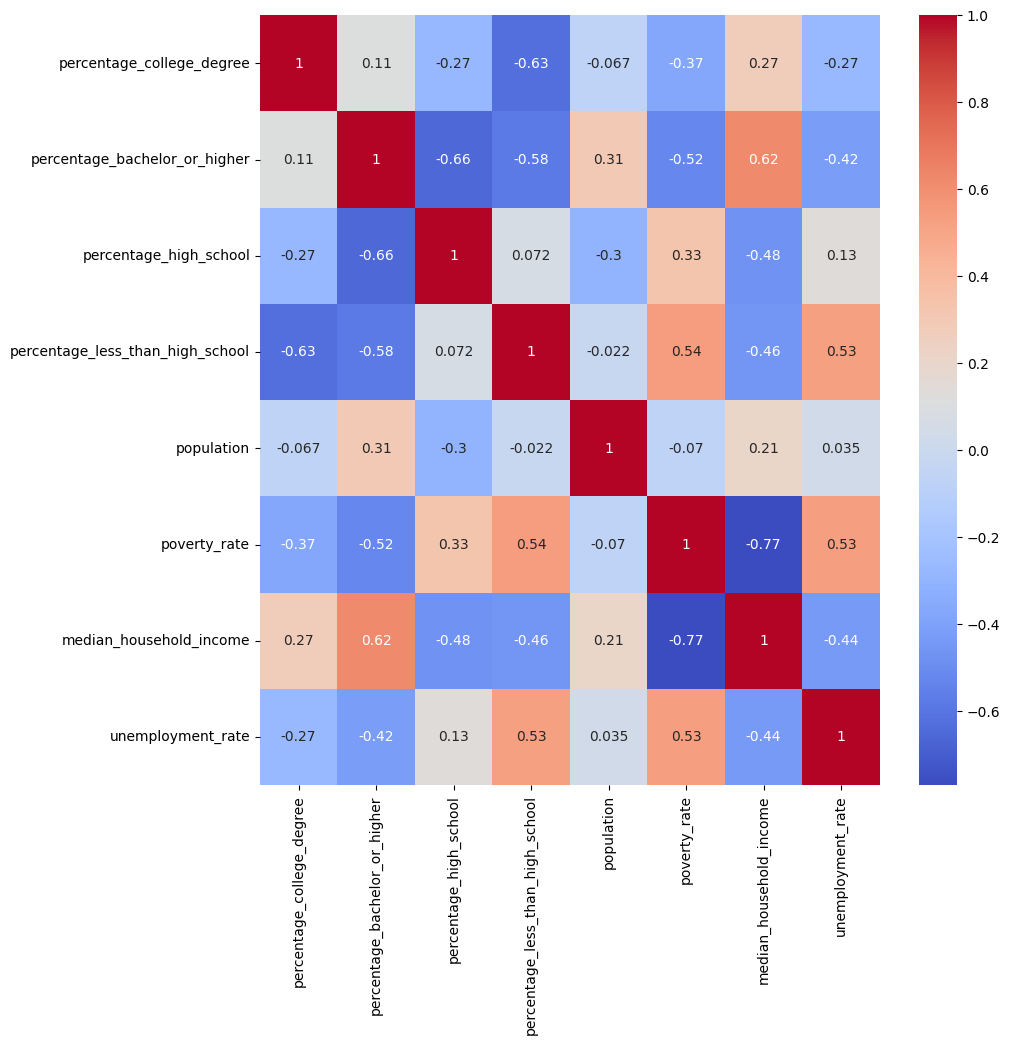
\includegraphics[width=0.7\textwidth]{images/CH03_Enrichment_Correlation.png}
    \caption{Correlation Between the Enrichment Features}
    \label{fig:CH03_Enrichment_Correlation}
\end{figure}